% !TEX program = tectonic
% FICHE BACKTEST HOUSE — A4 portrait, 2 colonnes, 9 étapes en 2 actes. Même gabarit que FICHE_DONNEES_HOUSE.
% RÈGLES DE FORME (identiques à la fiche données) :
%   · corps en \footnotesize partout ; \scriptsize gris pour les seules sources ; un chiffre-phare en
%     \Large par étape, aucune autre variation de taille.
%   · une étape = une boîte insécable au gabarit constant : titre + ruban, une phrase qui répond,
%     le chiffre-phare et son unité, deux à trois puces, un visuel, la source.
% RÈGLE DE FOND : on n'empile que des tests. Chaque étape dit ce qu'on CHANGE et ce qu'on OBSERVE.
%   Jamais « ça marche » ni « ça ne marche pas ». Le mot verdict n'apparaît pas.
% Chaque chiffre sort d'une cellule exécutée de Portefeuilles_House_Complet.ipynb (partie P5).
\documentclass[10pt,a4paper]{article}
\usepackage[margin=1.05cm]{geometry}
\usepackage[T1]{fontenc}
\usepackage[utf8]{inputenc}
\usepackage{lmodern}
\usepackage[french]{babel}
\usepackage{amsmath,amssymb}
\usepackage{booktabs}
\usepackage{multicol}
\usepackage{xcolor}
\usepackage{graphicx}
\usepackage{enumitem}
\usepackage{tikz}
\usepackage[most]{tcolorbox}
\usetikzlibrary{positioning}

\definecolor{bleu}{RGB}{20,77,144}
\definecolor{vert}{RGB}{20,110,60}
\definecolor{orange}{RGB}{196,123,0}
\definecolor{rouge}{RGB}{160,30,30}
\definecolor{grisf}{RGB}{110,110,110}
\definecolor{grisc}{RGB}{205,205,205}

\setlength{\columnsep}{5.5mm}
\setlength{\parindent}{0pt}
\setlength{\parskip}{0pt}
\pagestyle{empty}
\setlist[itemize]{leftmargin=3.4mm,topsep=0.9mm,itemsep=0.85mm,parsep=0pt,label=\textbullet}

\newcommand{\ruban}[1]{%
  \begin{tikzpicture}[baseline=-0.6ex, x=2.35mm, y=2.35mm]
    \foreach \k in {1,...,9}{%
      \ifnum\k=#1\relax
        \fill[white] (\k,0) circle (0.9);
      \else
        \fill[white, opacity=0.42] (\k,0) circle (0.6);
      \fi}
  \end{tikzpicture}}

\newtcolorbox{etapebox}[3]{%
  enhanced, breakable=false, colback=#2!3, colframe=#2!55, boxrule=0.5pt,
  arc=2pt, left=2.2mm, right=2.2mm, top=1.8mm, bottom=1.8mm,
  toptitle=0.7mm, bottomtitle=0.7mm, boxsep=0pt,
  title={\begin{minipage}[c]{0.63\linewidth}\raggedright\footnotesize\bfseries
           \textcolor{white}{#3}\end{minipage}\hfill
         \begin{minipage}[c]{0.30\linewidth}\raggedleft\ruban{#1}\end{minipage}},
  colbacktitle=#2, coltitle=white, fonttitle=\footnotesize\bfseries,
  before skip=1.9mm, after skip=0mm}

\newcommand{\reponse}[1]{{\footnotesize #1\par}\vspace{1.1mm}}
\newcommand{\phare}[3]{%
  \begin{center}\vspace{-0.6mm}
  {\Large\bfseries\color{#3} #1}\\[0.4mm]{\footnotesize #2}
  \end{center}\vspace{0.6mm}}
\newcommand{\pts}[1]{{\footnotesize\begin{itemize}#1\end{itemize}}\vspace{0.9mm}}
\newcommand{\vis}[1]{\vspace{0.8mm}\begin{center}\includegraphics[width=0.94\linewidth]{figures/#1}\end{center}\vspace{0.4mm}}
\newcommand{\src}[1]{{\scriptsize\color{grisf} #1\par}}
\newcommand{\acte}[2]{%
  \vspace{1.1mm}{\footnotesize\bfseries\color{#2} #1}\vspace{-1.3mm}
  \par{\color{#2}\rule{\linewidth}{1pt}}\vspace{0.6mm}}
\newlength{\colw}\setlength{\colw}{0.4865\textwidth}
\newcommand{\rangee}[2]{%
  \noindent\begin{minipage}[t]{\colw}\vspace{0pt}#1\end{minipage}%
  \hfill\begin{minipage}[t]{\colw}\vspace{0pt}#2\end{minipage}\par}

\begin{document}

% ═══════════════ CHAPEAU ═══════════════
\begin{center}
{\large\bfseries Copier les portefeuilles : la suite de tests}
\\[0.5mm]
{\scriptsize ce qu'on copie, comment, et ce qu'on observe $\cdot$ House 2014-2026
$\cdot$ notebook \texttt{Portefeuilles\_House\_Complet}, partie P5}
\end{center}
\vspace{1.4mm}

\begin{tcolorbox}[enhanced, colback=white, colframe=grisc, boxrule=0.5pt, arc=2pt,
                  left=3mm, right=3mm, top=1.5mm, bottom=1.5mm]
{\footnotesize\bfseries\color{bleu} ACTE I --- la règle du jeu}\hfill
{\footnotesize\bfseries\color{vert} ACTE II --- ce qu'on observe}\\[0.9mm]
\begin{center}
\begin{tikzpicture}[x=0.98cm, y=0.9cm, font=\scriptsize]
\foreach \k/\lab/\c [count=\i from 0] in {%
  1/un fonds/bleu, 2/qui est éligible/bleu, 3/le classement/bleu, 4/le capital/bleu,
  5/le réglage/vert, 6/année par année/vert, 7/combien copier/vert, 8/la source/vert, 9/la portée/vert}{%
  \ifnum\k<9 \draw[\c!45, line width=0.9pt] ({\i*2.1+0.28}, 0) -- ({\i*2.1+1.82}, 0);\fi
  \fill[\c] ({\i*2.1}, 0) circle (0.23);
  \node[text=white, font=\scriptsize\bfseries] at ({\i*2.1}, 0) {\k};
  \node[text=\c, font=\scriptsize, anchor=north] at ({\i*2.1}, -0.30) {\lab};}
\end{tikzpicture}
\end{center}
\vspace{0.2mm}
{\footnotesize\textbf{La règle du jeu, en une phrase.} On ne cherche pas à conclure : on \textbf{empile des
tests}, et chacun ne change \textbf{qu'un seul réglage}, toujours face au même repère --- le SPY, l'indice
des grandes actions américaines. La règle testée ici est la plus simple du projet : on classe les membres
par leur \textbf{Sharpe}, on copie les mieux classés, et on répartit le capital \textbf{à parts égales}.}
\end{tcolorbox}

\vspace{1.6mm}
% ═══════════════ ACTE I ═══════════════
\rangee{\begin{etapebox}{1}{bleu}{1 $\cdot$ UN MEMBRE EST UN FONDS}
\reponse{Le portefeuille reconstruit d'un membre a une valeur qui change chaque jour. Copier ce membre,
c'est acheter des parts de ce fonds : ni levier, ni vente à découvert.}
\phare{358}{membres copiables avec le dossier complet --- 226 avec les déclarations rapides seules}{bleu}
\vis{fig_10_valeur_part.png}
\pts{
\item La valeur de part vaut 1 au départ, puis suit les rendements quotidiens du portefeuille :
$\mathrm{NAV}_k(t) = \prod_{s \le t}(1 + r_k(s))$.
\item Elle ne dépend pas de la fortune du membre : on copie sa \emph{façon} d'investir, pas ses montants.
\item C'est la reconstruction de la fiche données qui rend ce fonds calculable : sans photo d'entrée,
un membre qui ne fait que vendre n'a aucun portefeuille à copier.
}
\src{source : cellule \og un membre = un fonds \fg{}. Exemple illustré : Brian Babin, le membre le plus souvent retenu.}
\end{etapebox}}{\begin{etapebox}{2}{bleu}{2 $\cdot$ QUI A LE DROIT D'ÊTRE COPIÉ}
\reponse{Deux conditions, vérifiées à chaque \textbf{coupe} --- le 31 décembre de chaque année, jour où
l'on refait le classement et où l'on redéploie le capital. Sans jamais regarder l'avenir : assez
d'historique, et un Sharpe au-dessus de 0,4.}
\phare{299}{membres éligibles l'année où le vivier est le plus large}{bleu}
\begin{center}\footnotesize
$\mathrm{Sharpe}_k = \dfrac{\overline{r_k}}{\sigma(r_k)}\sqrt{252}$
\qquad éligible si $n_{\text{jours}} \ge 126$ et $\mathrm{Sharpe} > 0{,}4$
\end{center}
\vspace{0.8mm}
\pts{
\item Le \textbf{Sharpe} rapporte le gain moyen à l'agitation du portefeuille : gagner 10 \% calmement
vaut mieux que gagner 10 \% en montagnes russes.
\item Le premier filtre (126 jours, soit six mois de bourse) écarte ceux qu'on ne connaît pas assez ; le
second écarte ceux dont le portefeuille n'a rien montré.
\item Aucun test statistique n'intervient ici. C'est un classement, pas une preuve.
}
\src{source : cellule \og le vivier \fg{}. Le vivier va de 54 membres (2015) à 299 (2025).}
\end{etapebox}}
\vfill
\rangee{\begin{etapebox}{3}{bleu}{3 $\cdot$ QUI ARRIVE EN TÊTE}
\reponse{Voici ce que la règle produit concrètement à une coupe : les mieux classés, le Sharpe qui les y
place, et l'historique sur lequel il est calculé.}
\phare{2,15}{le meilleur Sharpe à la coupe de fin 2021}{bleu}
\begin{center}\footnotesize
\begin{tabular}{@{}rlrr@{}}
\toprule
 & membre & Sharpe & jours \\
\midrule
1 & Peter Meijer & 2,15 & 245 \\
2 & Christopher L. Jacobs & 2,02 & 412 \\
3 & Victoria Spartz & 2,01 & 239 \\
4 & Abigail Spanberger & 1,93 & 150 \\
5 & Susan W. Brooks & 1,93 & 440 \\
\bottomrule
\end{tabular}\\[0.6mm]
{\footnotesize les cinq premiers sur 216 éligibles, dossier complet}
\end{center}
\vspace{0.8mm}
\pts{
\item Un Sharpe élevé peut reposer sur un historique court : c'est le prix du filtre à 126 jours, et il
est affiché ici plutôt que masqué.
\item Le classement est recalculé à chaque coupe : un membre peut y entrer une année et en sortir la
suivante.
}
\src{source : cellule \og le haut du classement à une coupe \fg{}.}
\end{etapebox}}{\begin{etapebox}{4}{bleu}{4 $\cdot$ COMMENT LE CAPITAL CIRCULE}
\reponse{À chaque coupe, trois gestes, toujours les mêmes. Rien n'entre, rien ne sort : le capital ne
bouge que par les mouvements de marché.}
\phare{3 gestes}{compter, redéployer, tenir --- répétés chaque année}{bleu}
\begin{center}\footnotesize
\textbf{(1) compter} \quad $W = \sum_k \mathrm{nbr}^k \, \mathrm{NAV}_k(t^R)$\\[0.8mm]
\textbf{(2) redéployer} \quad $\mathrm{nbr}^k = \dfrac{W/K}{\mathrm{NAV}_k(t^R)}$\\[0.8mm]
\textbf{(3) tenir} \quad pendant un an, sans y toucher
\end{center}
\vspace{0.8mm}
\pts{
\item $W$ est le capital du jour de la coupe, $K$ le nombre de membres copiés, $\mathrm{nbr}^k$ le nombre
de parts détenues chez le membre $k$.
\item Entre deux coupes, les poids \textbf{dérivent} : celui qui monte prend plus de place. C'est assumé,
et c'est ce qui distingue ce montage d'un rééquilibrage permanent.
\item Le fait que rien n'entre ni ne sort est vérifié automatiquement à chaque coupe.
}
\src{source : cellules \og le moteur en trois temps \fg{} et \og un bloc recalculé à la main \fg{}.}
\end{etapebox}}
\vfill
\newpage

% ═══════════════ ACTE II ═══════════════
\acte{ACTE II --- ce qu'on observe : un réglage change, une mesure suit}{vert}
\rangee{\begin{etapebox}{5}{vert}{5 $\cdot$ LE RÉGLAGE DE BASE}
\reponse{Le nombre de membres copiés n'est pas choisi à la main : chaque année on retient celui qui aurait
le mieux fonctionné sur le passé seulement. Voici ce que donne ce réglage.}
\phare{$+0{,}2$ \%}{d'écart au SPY par an, en moyenne sur 11 années}{vert}
\vis{fig_10_nav.png}
\pts{
\item Six années au-dessus du SPY, cinq en dessous.
\item Le nombre de membres copiés est choisi dans une grille de 4 à 20, sur le passé uniquement : aucune
information postérieure à la coupe n'entre dans la décision.
\item La courbe démarre à la première année tenue, 2016 : il faut une coupe pour classer, donc au moins
une année d'historique.
}
\src{source : cellule \og le réglage de base \fg{}. SPY = l'indice des grandes actions américaines,
dividendes réinvestis.}
\end{etapebox}}{\begin{etapebox}{6}{vert}{6 $\cdot$ ANNÉE PAR ANNÉE}
\reponse{Une année civile compte pour une observation. On compare ce que rapporte la stratégie et ce que
rapporte le SPY sur la même année.}
\phare{18 points}{entre la meilleure et la pire année}{vert}
\vis{fig_10_exces_annuel.png}
\pts{
\item Meilleure année : $+9$ \% en 2019. Pire : $-8$ \% en 2024.
\item Un tel écart entre les années dit à lui seul que la moyenne de $+0{,}2$ \% ne se lit pas sans son
incertitude : c'est l'objet de l'étape 9.
\item Onze observations, c'est le maximum disponible : la fenêtre de données commence en 2014 et la
première année tenue est 2016.
}
\src{source : cellule \og l'excès année par année \fg{}.}
\end{etapebox}}
\vfill
\rangee{\begin{etapebox}{7}{vert}{7 $\cdot$ COMBIEN DE MEMBRES COPIER}
\reponse{On change un seul réglage : le nombre de membres copiés, fixé cette fois de 4 à 20, et on regarde
ce que devient l'écart au marché.}
\phare{K = 6}{le nombre qui produit le plus grand écart mesuré}{vert}
\vis{fig_10_balayage_k.png}
\pts{
\item L'écart est maximal au milieu de la grille, pas au minimum : $K = 4$ donne $+0{,}7$ \%/an,
$K = 6$ donne $+1{,}4$ \%/an. Copier très peu ne fait pas grandir l'écart, cela le rend plus instable.
\item Au-delà de $K \approx 13$, l'écart s'inverse et devient négatif : $-2{,}0$ \%/an à $K = 20$.
\item Aucune valeur de $K$ ne fait franchir le seuil de 1,81 (étape 9) : le meilleur cas atteint
$t = 0{,}70$.
}
\src{source : cellule \og le balayage de K \fg{}, reconstruite depuis les blocs déjà calculés.}
\end{etapebox}}{\begin{etapebox}{8}{vert}{8 $\cdot$ LA SOURCE CHANGE-T-ELLE LE RÉSULTAT}
\reponse{Même règle, même moteur, quatre jeux de données : c'est la question de la fiche données
transposée à la stratégie.}
\phare{$-0{,}1$ \% à $+7{,}2$ \%}{l'écart annuel selon la source copiée --- pour un $t$ qui reste entre $-0{,}08$ et $0{,}88$}{vert}
\vspace{0.8mm}\begin{center}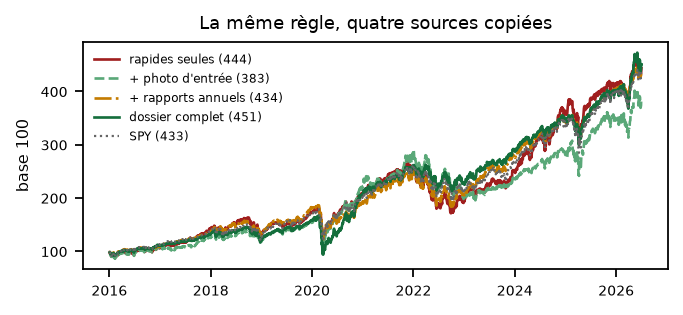
\includegraphics[width=0.82\linewidth]{figures/fig_10_sources.png}\end{center}\vspace{0.4mm}
\begin{center}\footnotesize
\begin{tabular}{@{}lrrrr@{}}
\toprule
source copiée & écart/an & $t$ & $\beta$ & $\alpha$/an \\
\midrule
déclarations rapides seules & $+0{,}9$ \% & $0{,}37$ & $0{,}99$ & $+0{,}6$ \% \\
$+$ photo d'entrée & $+7{,}2$ \% & $\mathbf{0{,}88}$ & $0{,}99$ & $+5{,}5$ \% \\
$+$ rapports annuels & $-0{,}1$ \% & $-0{,}08$ & $0{,}91$ & $+1{,}1$ \% \\
dossier complet & $+0{,}2$ \% & $0{,}13$ & $0{,}93$ & $+1{,}2$ \% \\
\bottomrule
\end{tabular}
\end{center}
\vspace{0.8mm}
\pts{
\item Ajouter la photo d'entrée change le point de départ de chaque membre, donc son historique et son
classement ; ajouter les rapports annuels ajoute des membres entiers, ceux qu'on ne voyait pas du tout.
\item L'écart annuel, lui, bouge beaucoup : la ligne \emph{$+$ photo d'entrée} affiche $+7{,}2$ \%/an
contre $-0{,}1$ \% pour les rapports annuels. Mais son $t$ reste à $0{,}88$, sous le seuil de l'étape 9.
\item \textbf{Pourquoi} : ce $+7{,}2$ \% tient à une seule année. En 2020, cette ligne fait $+87$ points ;
les dix autres années restent entre $-7$ et $+13$. Une moyenne portée par une année ne se lit pas comme un
écart régulier --- c'est précisément ce que le $t$ mesure.
}
\src{source : cellule \og le réglage de base \fg{}, quatre jeux de données.}
\end{etapebox}}
\vfill
\vspace{3mm}
\rangee{\begin{etapebox}{9}{vert}{9 $\cdot$ CE QU'ON PEUT AFFIRMER}
\reponse{Quatre mesures, et ce que chacune dit exactement. Puis la question qu'aucune ne règle : avec onze
années, qu'aurait-on été capable de détecter ?}
\phare{4,8 \%}{l'écart annuel minimal détectable huit fois sur dix}{vert}
\pts{
\item \textbf{L'écart annuel moyen} dit de combien on bat le SPY, en moyenne.
\item \textbf{Le $t$} rapporte cet écart à sa propre instabilité. Au-delà de $|t| \approx 1{,}81$, un
écart de cette taille serait rare si la stratégie ne valait pas mieux que le marché. Ici, le plus haut
mesuré est $0{,}88$.
\item \textbf{Le $\beta$} mesure la part du mouvement qui suit simplement le marché. Un $\beta$ supérieur
à 1 signifie qu'on prend plus de risque de marché : le gain vient alors du risque, pas de la sélection.
\item \textbf{L'$\alpha$} est ce qui reste une fois le marché retiré. C'est la seule mesure qui isole
l'apport propre du choix des membres.
\item \textbf{La portée du test} : avec 11 années et une instabilité de 5,9 \% par an, un écart réel
inférieur à 4,8 \% par an serait resté invisible huit fois sur dix. Un $t$ faible borne donc ce qu'on peut
voir --- il ne prouve pas qu'il n'y a rien.
}
\src{source : cellules \og les mesures \fg{} et \og la puissance du test \fg{}.}
\end{etapebox}}{\begin{tcolorbox}[enhanced, breakable=false, colback=rouge!3, colframe=rouge!45, boxrule=0.5pt,
                  arc=2pt, left=2.2mm, right=2.2mm, top=1.8mm, bottom=1.8mm,
                  toptitle=0.7mm, bottomtitle=0.7mm, boxsep=0pt, before skip=1.9mm, after skip=0mm,
                  colbacktitle=rouge, coltitle=white, fonttitle=\footnotesize\bfseries,
                  title={CE QUE CETTE SUITE DE TESTS NE DIT PAS}]
\reponse{Cette première version est volontairement la plus simple possible. Cinq choses n'y sont pas, et
chacune peut changer les chiffres ci-contre.}
\pts{
\item \textbf{Les transactions entrent à leur date d'opération}, pas à leur date de publication. Un
suiveur réel agirait 27 jours plus tard sur les déclarations rapides, et plus d'un an plus tard sur les
rapports annuels. Ce qui est mesuré ici est donc une \textbf{borne haute}.
\item \textbf{Aucun coût de transaction} n'est appliqué. Redéployer le capital chaque année en coûte.
\item \textbf{Aucun placebo} n'est joué : on ne vérifie pas ici ce que donnerait la même règle sur des
membres tirés au hasard.
\item \textbf{Une seule façon de répartir le capital} est testée, à parts égales.
\item \textbf{Une seule règle de classement}, le Sharpe --- celle que le deck de données désigne comme la plus simple.
}
{\footnotesize\textbf{Ce que la suite établit quand même.} Une trace : à chaque réglage changé, une mesure,
toujours face au même repère. Et la vérification de la fiche données reste le juge indépendant : elle dit
si la reconstruction colle aux déclarations des élus, que la stratégie gagne ou non.}
\end{tcolorbox}}
\vspace{2.5mm}

\begin{tcolorbox}[enhanced, colback=white, colframe=grisc, boxrule=0.5pt, arc=2pt,
                  left=3mm, right=3mm, top=1.6mm, bottom=1.6mm,
                  colbacktitle=grisf, coltitle=white, fonttitle=\footnotesize\bfseries,
                  title={LA TRACE --- ce qu'on a changé, ce qu'on a observé}]
\begin{center}\footnotesize
\begin{tabular}{@{}llll@{}}
\toprule
étape & on teste\ldots & ce qu'on change & ce qu'on observe \\
\midrule
1-4 & la règle du jeu & --- (la règle est posée) & 358 membres copiables \\
5 & le réglage de base & rien : c'est la référence & $+0{,}2$ \%/an, $t = 0{,}13$ \\
6 & année par année & rien & 6 années sur 11 au-dessus du SPY \\
7 & combien copier & le nombre $K$, de 4 à 20 & meilleur cas $K = 6$, $t = 0{,}70$ \\
8 & la source copiée & les 4 jeux de données & $t$ de $-0{,}08$ à $0{,}88$ \\
9 & la portée du test & rien & écart détectable : 4,8 \%/an \\
\bottomrule
\end{tabular}
\end{center}
\vspace{0.6mm}
{\footnotesize On lit \emph{ce qu'on change} et \emph{ce qu'on observe} : une trace, pas une sentence.
Aucune configuration testée n'atteint le seuil de 1,81 ; la plus haute vaut 0,88. Et l'étape 9 borne la
lecture : sous 4,8 \% par an, un écart réel serait probablement resté invisible avec onze années.}
\end{tcolorbox}

\end{document}
